\subsection{Build pipeline}
\label{sec:structure-buildpipeline}
After the HTTP- and authentication service was built as a user interaction possibility for the upcoming build pipeline realization, the full extent of the necessary API endpoints needed to be defined. Since the OAuth 2.0 framework was already implemented and the access to the GitHub API was prepared as includeable module, only the endpoints responsible for managing and triggering builds, needed to be reserved for the final build service development.

\subsubsection{API integration}

%% Graphic of the first draft of the API
\begin{figure} % h-ere, t-op, b-ottom, p-age
    \centering
    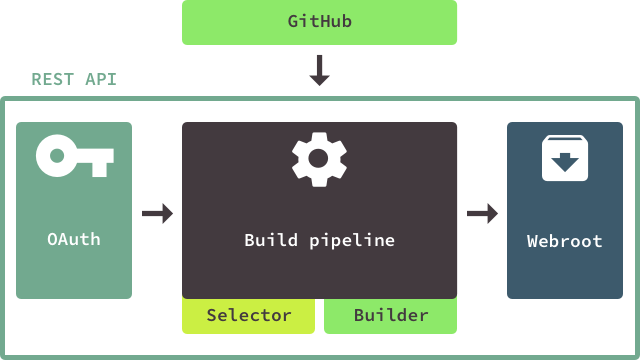
\includegraphics[width=0.9\textwidth]{buildpipeline-api.png}
    \caption{A graphic showing the first draft of the then proposed API cycle. At first the OAuth step should care for authentication, then the build pipeline should be initiated and orchestrate its services to interact with the GitHub API, select files to build and run the build task before saving a rendered version of the webroot, ready for deployment.}
    \label{fig:buildpipeline-api}
\end{figure}
%

From the first draft of an API cycle (as seen in fig. \ref{fig:buildpipeline-api}) to the final structure, a lot of details needed to be tidied up. This was mainly due to the complexity of the build pipeline itself, since one of the biggest challenges were to provide a real non-blocking event loop. By realizing such a non-blocking loop, the client receives an instant, intermediate response, instead of having to queue beforehand, and/or wait until the whole operation finishes. Furthermore, a recurring request for obtaining the build status was enabled using an own endpoint returning informations from the database entry.

The endpoints, which were implemented in favor of user projects, were the following:

\begin{itemize}
  \item \texttt{POST /api/project} -- Creates a project in the database, together with reference to its GitHub data.
  \item \texttt{POST /api/project/:owner/:repo/delete} -- Deletes all references to the project from the database.
  \item \texttt{POST /api/project/:owner/:repo/build} -- Trigger a new build cycle. Returns the reference to the database entry of its build log.
  \item \texttt{GET /api/project/:owner/:repo/status} -- Get the status of the latest build (pending, failed, success).
  \item \texttt{GET /api/project/:owner/:repo/download} -- Download the latest successful build as tar.gz-archive. (e.g. for automated deployments)
\end{itemize}

\subsubsection{Tasks}
As already explained, the build pipeline is realized as a modular concept, consisting of different sub-tasks, bound together in a network of various dependencies to and from each other. Most of these modules are dynamically interlinked with API calls to GitHub, but also with partially strong data modifications of the respective responses.

One after the other, all necessary modules are loaded on request -- to not confuse them by their actual functions, they are divided into three action levels: \emph{engine}, \emph{module} and \emph{support}.

\begin{itemize}
  \item Engine-specific tasks are immediately working for and on the compile actions (e.g. setting up the build pipeline, loading necessary modules, etc\ldots),
  \item Module-specific tasks care for external assistance (e.g. installing modules, compressing rendered output, etc\ldots) and
  \item Support-specific tasks care for engine-specific assistance (e.g. parsing configurations, creating new database entries, etc\ldots).
\end{itemize}
